\tikzset{
    neuron/.style={
		circle,
		draw=black,
		minimum size=0.8cm,
		fill=gray,
	},	
    neuron dark/.style={
		circle,
		draw=black,
		minimum size=0.8cm,
		fill=TUMBlueDark,
	},	
	neuron missing/.style={
		draw=none, 
		fill=white,
		scale=1.0,
		text height=0.3cm,
		execute at begin node=\color{black}$\vdots$
	},
	neuron sigma/.style={
		circle,
		draw=black,
		fill=white,
		scale=1.0,
%		text height=0.5cm,
		execute at begin node=\color{black}$\Sigma$
	},	
	label/.style = {draw=none, fill=none, rectangle, minimum height=1em, minimum width=1em},
	blockrx/.style = {draw, fill=white, rectangle, minimum height=1.5em, minimum width=6.25em},
	blocktx/.style = {draw, fill=white, rectangle, minimum height=1.5em, minimum width=13em},
	block/.style = {draw, fill=white, rectangle, minimum height=2em, minimum width=10em,rounded corners},
	blockthesis/.style = {draw, fill=gray!20, rectangle, minimum height=1.5em, minimum width=40em,rounded corners},
	block1/.style = {draw, fill=white, rectangle, minimum height=1.5em, minimum width=1.5em,rounded corners},
	tmp/.style  = {coordinate}, 
	sum/.style= {draw, fill=white, circle, node distance=1cm},
	mul/.style= {draw=none, fill=white, circle, node distance=1cm},
	input/.style = {coordinate},
	output/.style= {coordinate},
	pinstyle/.style = {pin edge={to-,thin,black}
	}
}
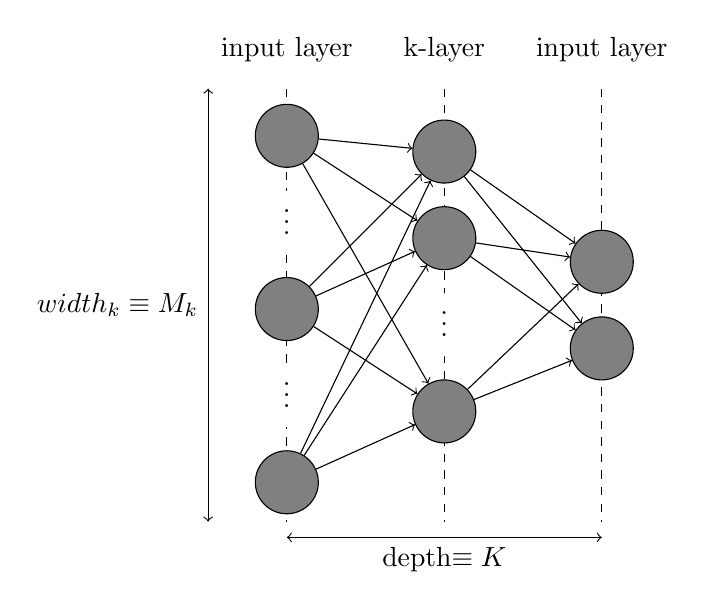
\begin{tikzpicture}
	\draw [<->] (-1,1.5) -- (-1,-4) node [left, midway] {$\text{width}_k\equiv M_k$};	

	\draw [dashed] (0,1.5) -- (0,-4) node [yshift=6cm] {input layer};
	
	\foreach \m [count=\y] in {1,missing,3,missing,5}
	\node [neuron/.try, neuron \m/.try] (input1-\y) at (0,2-\y*1.1) {};
	
	\draw [dashed] (2,1.5) -- (2,-4) node [yshift=6cm] {k-layer};
	
	\foreach \m [count=\y] in {1,2,missing,4}
	\node [neuron/.try, neuron \m/.try ] (hidden1-\y) at (2,1.8-\y*1.1) {};
	
	\draw [dashed] (4,1.5) -- (4,-4) node [yshift=6cm] {input layer};	
	
	\foreach \m [count=\y] in {1,2}
	\node [neuron/.try, neuron \m/.try ] (output1-\y) at (4,0.4-\y*1.1) {};
	
	\draw [<->] (0,-4.2) -- (4,-4.2) node [below, midway] {depth$\equiv K$};	

	%mesh1
	\foreach \i in {1,3,5} 
	\foreach \j in {1,2,4}
	\draw [->] (input1-\i) -- (hidden1-\j);
	
	
	\foreach \i in {1,2,4}
	\foreach \j in {1,2}
	\draw [->] (hidden1-\i) -- (output1-\j);
	
\end{tikzpicture}